% template created by: Russell Haering. arr. Joseph Crop
\documentclass[12pt]{article}
\usepackage[hmargin=1in, vmargin=1in]{geometry}
\usepackage{fancyhdr}
\pagestyle{fancy}
\usepackage[hang,small]{caption}
\usepackage{lastpage}
\usepackage{graphicx}
\usepackage{verbatim}
\DeclareGraphicsExtensions{.jpg}
\usepackage{url}

\def\author{Jacques Uber and Kevin Ngo}
\def\title{ECE472 Lab4 Report}
\def\date{\today}

\fancyhf{}
\fancyhead[LO]{\author}
\fancyhead[RO]{\date}
\fancyfoot[C]{\thepage\
                    / 7}

                    \setcounter{secnumdepth}{0}
                    \setlength{\parindent}{0pt}
                    \setlength{\parskip}{4mm}
                    \linespread{1.4}

\begin{document}

\fancyhf{}
\fancyhead[LO]{\author}
\fancyhead[RO]{\date}
\fancyhead[CO]{\title}

\section{Lab Report}
In this lab, we modify a MIPS single-cycle processor's datapath and control
signals to handle the JUMP, ADDI, BEQ, and BNE instructions.

\begin{enumerate}
    \item
    Waveform diagram of the JUMP instruction.
    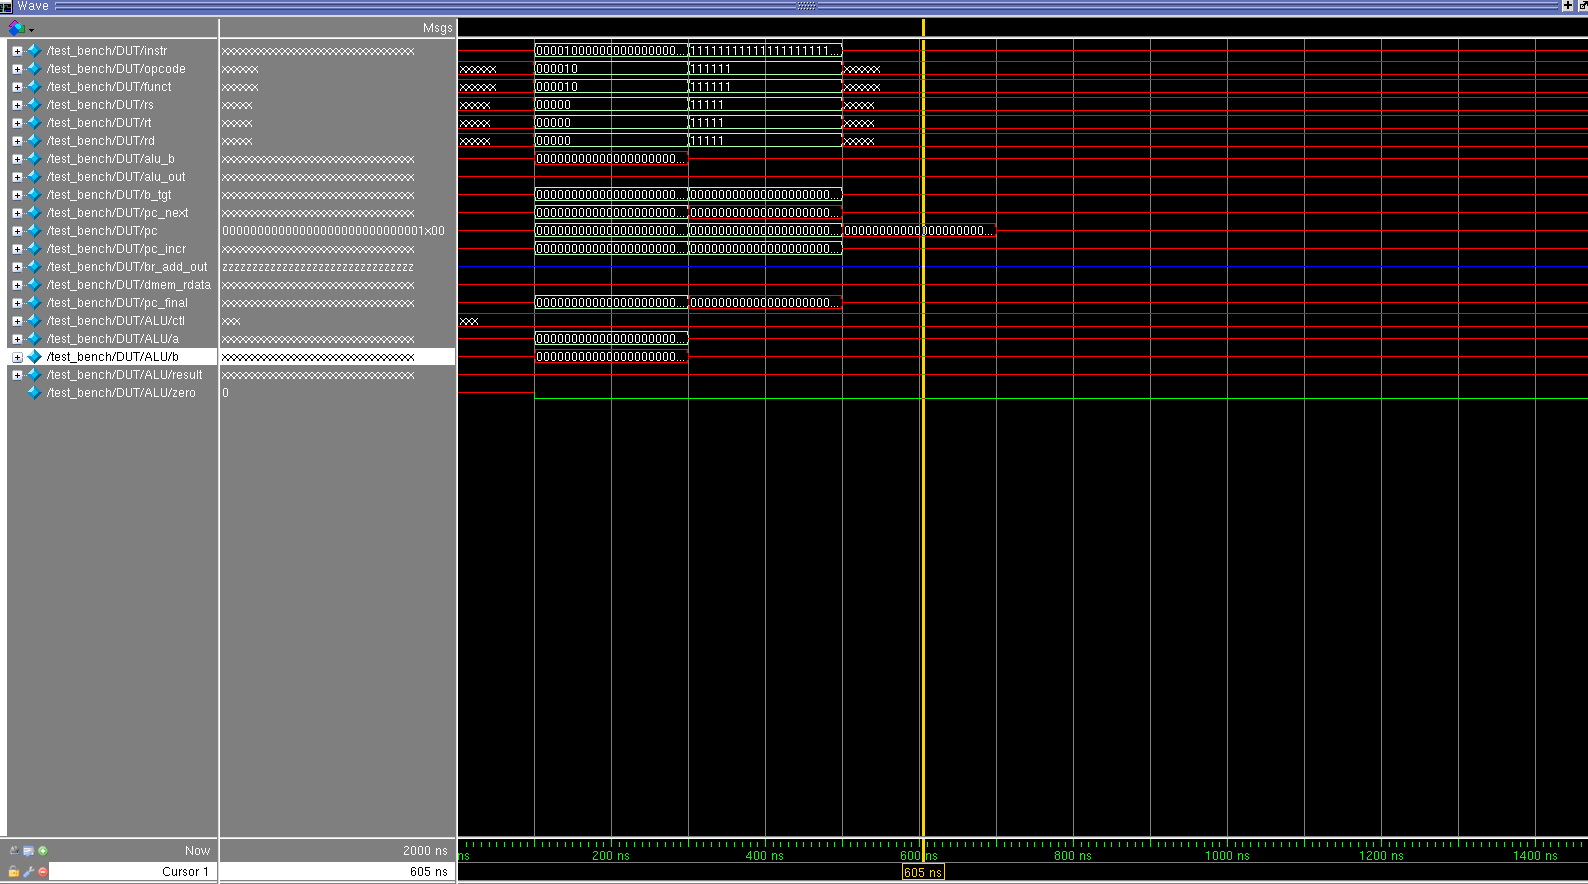
\includegraphics[scale=0.55]{img/jump_wave.png}

    \item
    Waveform diagram of the ADDI instruction.
    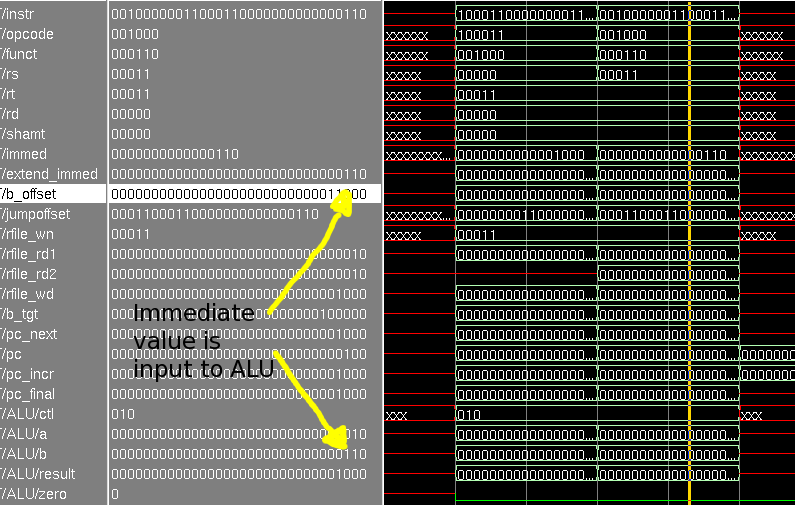
\includegraphics[scale=0.55]{img/addi_wave.png}

    \item
    Waveform diagram of the BEQ instruction.
    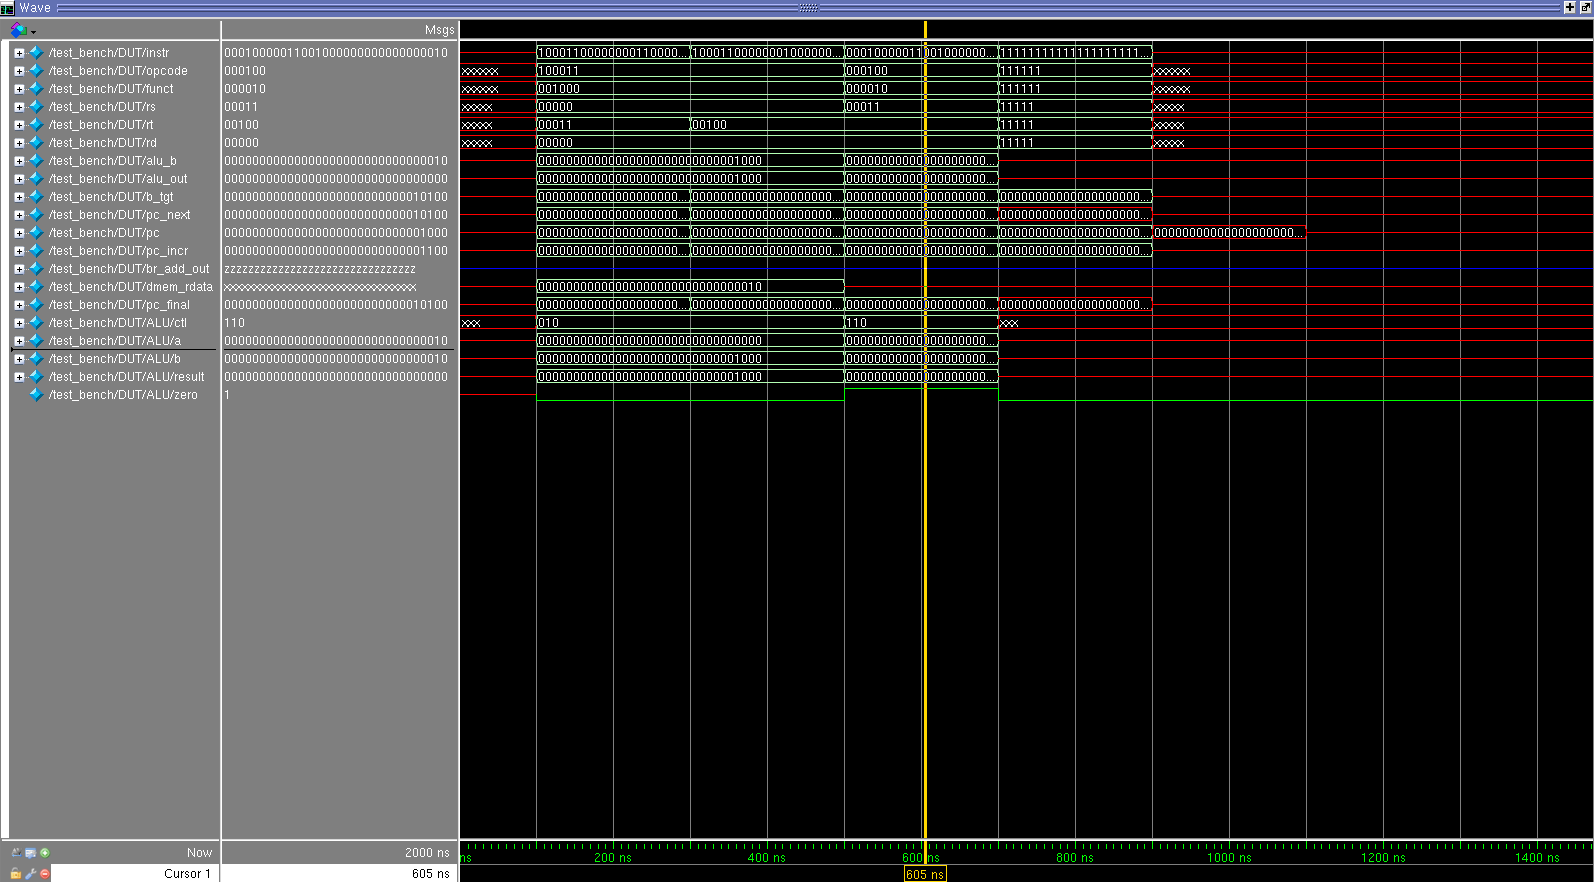
\includegraphics[scale=0.55]{img/beq_wave.png}

    \item
    Waveform diagram of the BNE instruction.
    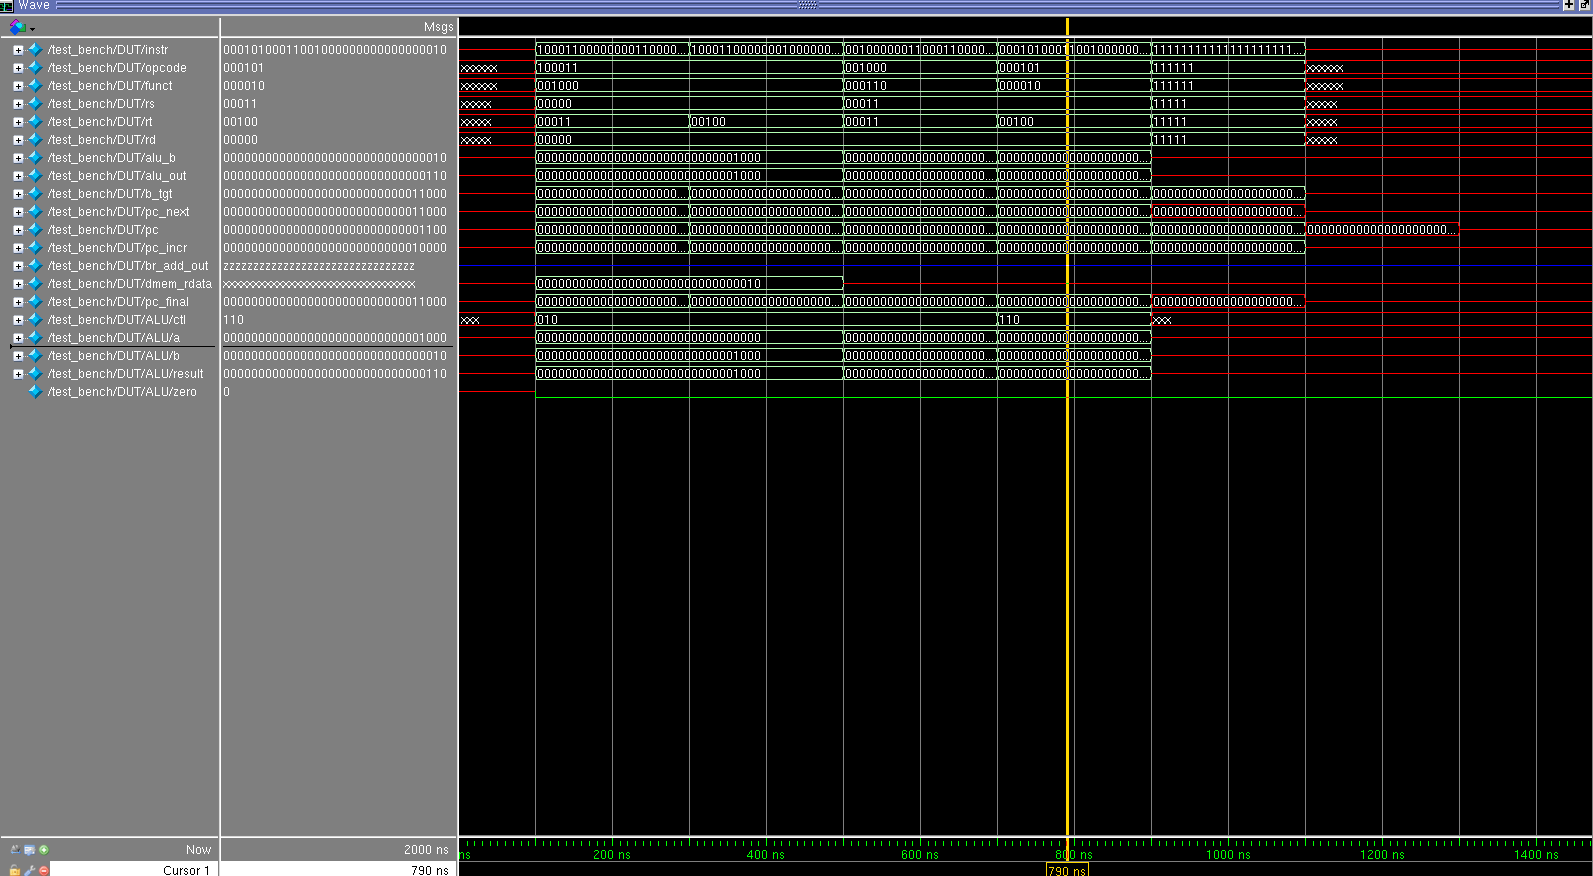
\includegraphics[scale=0.55]{img/bne_wave.png}

    \item
    Waveform diagram of the test assembly program.
    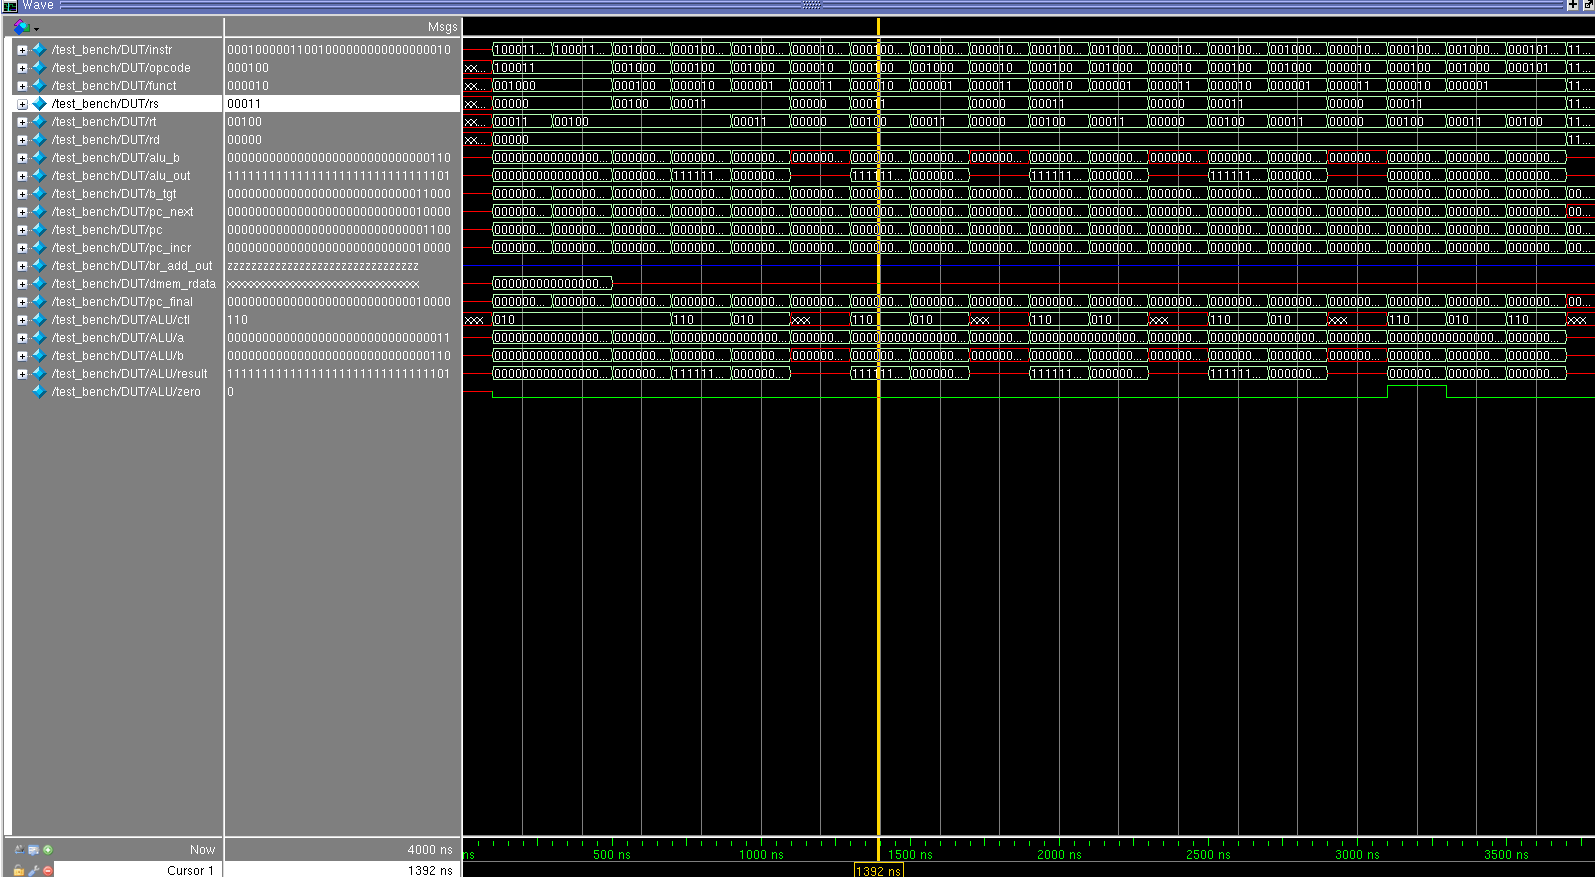
\includegraphics[scale=0.55]{img/test_program_wave.png}
\end{enumerate}

\section{Lab Code}
{\tiny
\begin{verbatim}

\end{verbatim}
}

\end{document}
